\chapter{Search for Resonances in the Resolved Dijet Final State with an Initial State Radiation}
\label{chapter:dijetISR}


\epigraph{\textit{It is our perpetual dissatisfaction with ourselves that causes us to approach the world as a space of possibility that has the power to awaken our attention and make us marvel at its vibrant details.}}{― Mari Ruti, A World of Fragile Things: Psychoanalysis and the Art of Living}

%\epigraph{\textit{The bud disappears in the bursting-forth of the blossom, and one might say that the former is refuted by the latter; similarly, when the fruit appears, the blossom is shown up in its turn as a false manifestation of the plant, and the fruit now emerges as the truth of it instead.
%}}{--Georg Wilhelm Friedrich Hegel, Phenomenology of Spirit}

This chapter is heavily based on work previously published~\cite{dijetISR2019}in collaboration with ATLAS.

\section{Introduction}

%\newcommand{\pT}{\ensuremath{p_{\text{T}}}\xspace}
\newcommand{\pt}{\ensuremath{p_{\text{T}}}\xspace}
\newcommand{\MGMCatNLOV}[1]{\textsc{MadGraph5}\_aMC@NLO~#1\xspace}
\newcommand{\PYTHIA}{\textsc{Pythia}\xspace}

%\newcommand{\pt}{\ensuremath(P_{T})}
\newcommand{\ifb}{\ensuremath(ifb)}
\newcommand{\ptmin}{\ensuremath{\pt^{\textrm{min}}}\xspace}
\newcommand{\nphoton}{\ensuremath{n_{\gamma}}\xspace}
\newcommand{\photonPt}{\ensuremath{E_{\textrm{T}}^{\gamma}}\xspace}
\newcommand{\jetPt}{\ensuremath{p_{\textrm{T}}^{\textrm{jet}}}\xspace}
\newcommand{\ntag}{\ensuremath{n_{\textrm{$b$-tag}}}\xspace}
\newcommand{\mjj}{\ensuremath{m_{\textrm{jj}}}\xspace}
\newcommand{\yStar}{\ensuremath{y^{\ast}}\xspace}
\newcommand{\jetEta}{\ensuremath{\eta^{\textrm{jet}}}\xspace}

\newcommand{\photonPtTrig}{\ensuremath{E_{\textrm{T, trig}}^{\gamma}}\xspace}
\newcommand{\photonEta}{\ensuremath{\eta^{\gamma}}\xspace}
\newcommand{\photonY}{\ensuremath{y^{\gamma}}\xspace}
\newcommand{\photonPhi}{\ensuremath{\phi^{\gamma}}\xspace}
\newcommand{\jetEt}{\ensuremath{E_{\textrm{T}}^{\textrm{jet}}}\xspace}

\newcommand{\jetY}[1]{\ensuremath{y_{#1}^{\textrm{jet}}}\xspace}
\newcommand{\jetPhi}{\ensuremath{\phi^{\textrm{jet}}}\xspace}
\newcommand{\njet}{\ensuremath{n_{\textrm{jets}}}\xspace}
\newcommand{\gq}{\ensuremath{g_{\textrm{q}}}\xspace}
\newcommand{\Zprime}{\ensuremath{Z^{\prime}}\xspace}
\newcommand{\lumiRange}{\ensuremath{76.6\textrm{--}79.8\,\ifb}\xspace}
\newcommand{\btagged}{\ensuremath{b}-\textrm{tagged}}
\newcommand{\btagging}{\ensuremath{b}-\textrm{tagging}}
\newcommand{\BumpHunter}{BumpHunter\xspace}

\newcommand{\MassRangeSingle}{\textcolor{red}{$169\,\GeV$\textrm{--}$300\,\GeV$}\xspace}
\newcommand{\MassRangeCompound}{\textcolor{red}{$300\,\GeV$\textrm{--}$X\,\GeV$}\xspace}
\newcommand{\ApproxMassRangeGamma}{\ensuremath{225~\GeV}\textrm{--}\ensuremath{1.1~\TeV}}
\newcommand{\FitStartGamma}{169~\GeV}
\newcommand{\FitStartJet}{303~\GeV}
%\newcommand{\LikHpvalGamma}{XXX\xspace} %not found in COM
\newcommand{\ChipvalGamma}{0.58\xspace}
\newcommand{\BHintervalGamma}{861~\GeV\textrm{--}917~\GeV}%consistent with figure 38 text in COM is obsolete
\newcommand{\BHpvalGamma}{0.67\xspace}%consistent with figure 38 text in COM is obsolete
%\newcommand{\LikHpvalJet}{XXX\xspace} % not found in COM
\newcommand{\ChipvalJet}{0.90\xspace} 
\newcommand{\BHintervalJet}{482~\GeV\textrm{--}523~\GeV}
\newcommand{\BHpvalJet}{0.6\xspace}

\newcommand{\SignalAcceptanceForMassPointGamma}{22}
\newcommand{\SignalAcceptanceForMassPointJet}{13} 

\newcommand{\cutcomment}{In the single-photon case all jets pass the leading and subleading jet requirements, since only jets above $25\,\GeV$ are considered eligible for the analysis}

\let\oldTeV\TeV
\let\oldGeV\GeV
\renewcommand{\TeV}{\oldTeV\xspace}
\renewcommand{\GeV}{\oldGeV\xspace}


% \newcommand{\ZprimeLimitStatement}{for masses $m_{\Zprime}$ of 250~\GeV and $\approx$400--550~\GeV, for couplings values of $\gq\sim 0.3$ and larger}
%\newcommand{\PhotonGaussianLimitStatement}{from approximately 340~fb at a mean mass of 250~\GeV to approximately 6~fb at 1.2~\TeV}
\newcommand{\PhotonGaussianLimitStatement}{from approximately 100--150~fb at a mean mass of 200~\GeV to approximately 10--20~fb at 1.2~\TeV}
\newcommand{\JetGaussianLimitStatement}{from approximately 100~fb at a mean mass of 350~\GeV to approximately 50~fb at 550~\GeV}
\newcommand{\JetZprimeLimitStatement}{\textbf{To be updated} for $\gq$ above 0.20 at mass $m_{\Zprime}=350$~\GeV and $\gq$ above 0.22 at $m_{\Zprime}=550$~\GeV}

Searches for resonant enhancements of the dijet invariant mass distribution (\mjj) are an essential part of the LHC physics programme.
%New particles produced directly in LHC collisions must interact with the constituent partons of the proton, and they may also decay to partons in the final state.
New particles with sizeable couplings to quarks and gluons are predicted by many models, such as those including resonances with additional couplings to dark-matter particles~\cite{Chala:2015ama,LHCDMF:2015}.

Searches for dijet resonances with masses of several hundreds of \GeV to just above 1~\TeV have been carried out at lower-energy colliders~\cite{Arnison:1983dk,Albajar:1988rs,Bagnaia1984283, Aaltonen:2008dn,Alitti:1990kw} and at the LHC, which has also extended search sensitivities into the multi-$\TeV$ mass range~\cite{EXOT-2010-01,CMS-EXO-10-010,CMS-QCD-10-016,CMS-EXO-11-015,EXOT-2010-07,EXOT-2011-07,EXOT-2011-21,EXOT-2013-11,CMS-EXO-12-016,EXOT-2015-02,CMS-EXO-13-001,CMS-EXO-16-056,CMS-EXO-16-032,EXOT-2016-20,EXOT-2016-21}.
Despite using higher integrated luminosities than earlier colliders, these LHC searches have been limited at lower masses by a large multi-jet background. 
Multi-jet events are produced at such high rates that fully recording every event would saturate the online data selection (called \textit{trigger}) and data acquisition systems.
To avoid this, minimum transverse momentum ($\ptmin$) thresholds are imposed on triggers collecting events with at least one jet (called single-jet triggers).
These thresholds create a lower bound on the sensitivity of searches 
%using these triggers 
at a mass of approximately $\mjj \approx 2\ptmin$, where $\ptmin$ is typically several hundred $\GeV.$
Consequently, searches for dijet resonances at the LHC have poor sensitivity for masses below $1\,\TeV$, and set limits on the couplings of the resonance to quarks in this light-resonance region which are weaker than limits in heavy-resonance regions~\cite{Dobrescu:2013coa}.
Nevertheless, despite the difficulty of recording events containing light resonances, they remain a viable search target at the LHC, both from a model-agnostic point of view~\cite{Harris:2011bh} and, for example, in models of spin-dependent interactions of quarks with dark matter~\cite{Chala:2015ama,LHCDMF:2015}. 

Recently, ATLAS and CMS have published searches for low-mass dijet resonances using several complementary strategies to avoid trigger limitations.
For $\mjj~>~450\,\GeV$, the most stringent limits are set by searches recording only partial event information~\cite{CMS-EXO-16-032,EXOT-2016-20}.

Another search avenue is opened by data in which a light resonance is boosted in the transverse direction via recoil against a high-$\pt$ photon~\cite{An:2012ue,Shimmin:2016vlc}.
Requiring a high-\pT photon in the final state reduces signal acceptance but allows efficient recording of events with lower dijet masses.
At even lower resonance masses, the decay products of the resonance will merge into a single large-radius jet. 
Searches for this event signature have been used to set limits on resonant dijet production at both ATLAS~\cite{EXOT-2017-01} and CMS~\cite{CMS-EXO-17-001,Sirunyan:2018ikr}.
However, these searches become less sensitive above $200\,\GeV$--$350\,\GeV$, when the decay products fall outside the large-radius jet cone.
%% btagged: EXOT-2016-33, goes to 0.57 TeV
%% TLA: EXOT-2016-20, goes to 0.45 TeV
%% Boosted: EXO-17-001, goes up to 0.22 TeV

This chapter presents a new search for resonances in events containing a dijet and a high-\pT photon in the final state, using proton--proton ($pp$) collisions recorded at a centre-of-mass energy $\sqrt{s} =$ 13~\TeV and corresponding to an integrated luminosity up to 79.8~\ifb.
The search targets a dijet mass range of \ApproxMassRangeGamma.
This range covers masses below the range accessible using single-jet triggers or partial-event data and above the mass range where the resonance decay products merge.
The search is performed using samples of events selected either with or without criteria designed to identify jets originating from bottom quarks (\textit{$b$-jets}).
Searching in a subset of the data selected with $b$-jet identification criteria enhances sensitivity to resonances which preferentially decay into bottom quarks.
This search probes masses above $225\,\GeV$, obtaining results complementary to the reach of previous dijet searches at a centre-of-mass energy of $\sqrt{s} =$ 13~\TeV: below approximately $600\,\GeV$, previous ATLAS di-$b$-jet searches lose sensitivity~\cite{EXOT-2016-33}, while the range of the CMS boosted di-$b$-jet search~\cite{Sirunyan:2018ikr} is limited to a mass region up to 350~\GeV. Another complementary CMS search for resonances with masses above $325\,\GeV$ decaying to $b$-jets at a centre-of-mass energy of $\sqrt{s} =$ 8~\TeV is described in Ref.~\cite{CMS-EXO-16-057}.

%% A complementary search, recording only partial event data in order to efficiently trigger on dijet events without requiring an ISR object, has been performed also focusing on light resonances with dijet masses of 425~\GeV--1.05~\TeV~in ATLAS~\cite{tla} and with dijet masses of 450~\GeV--1.6~\TeV~in CMS~\cite{Khachatryan:2016ecr}. Another recent complementary search for resonances with masses of 600~\GeV and above decaying to heavy-flavour jets is described in Ref.~\cite{lowMassDiB}.

%-------------------------------------------------------------------------------
%\section{ATLAS detector}
%%% \label{sec:detector}
%%-------------------------------------------------------------------------------
%\newcommand{\AtlasCoordFootnote}{ATLAS uses a right-handed coordinate system with its origin at the nominal interaction point (IP) in the centre of the detector and the $z$-axis along the beam pipe.
%The $x$-axis points from the IP to the centre of the LHC ring, and the $y$-axis points upwards.
%Cylindrical coordinates $(r,\phi)$ are used in the transverse plane, with $\phi$ being the azimuthal angle around the $z$-axis.
%The pseudorapidity is defined in terms of the polar angle $\theta$ as $\eta = -\ln \tan(\theta/2)$.
%It is equivalent to the rapidity for massless particles. 
%Transverse momentum and energy are defined as $\pt\equiv p \sin{\theta}$ and $\ET\equiv E \sin{\theta}$, respectively.
%Angular distance is measured in units of $\Delta R \equiv \sqrt{(\Delta\eta)^{2} + (\Delta\phi)^{2}}$.}
%
%The ATLAS experiment~\cite{PERF-2007-01,Capeans:1291633,CERN-LHCC-2012-009,Abbott:2018ikt} at the LHC is a multipurpose particle detector with a forward--backward symmetric cylindrical geometry\footnote{\AtlasCoordFootnote\xspace} with layers of tracking, calorimeter, and muon detectors over nearly the entire solid angle around the $pp$ collision point.
%The directions and energies of high transverse momentum particles are measured using tracking detectors, finely segmented hadronic and electromagnetic calorimeters, and a muon spectrometer, within axial and toroidal magnetic fields.
%The inner tracker consists of silicon pixel, silicon microstrip, and transition radiation tracking detectors, and reconstructs charged-particle tracks in $|\eta| < 2.5$.
%Lead/liquid-argon (LAr) sampling calorimeters provide electromagnetic (EM) energy measurements with high granularity.
%A steel/scintillator-tile hadronic calorimeter covers the central pseudorapidity range ($|\eta| < 1.7$).
%The endcap and forward regions are instrumented with LAr calorimeters for EM and hadronic energy measurements up to $|\eta| = 4.9$.
%The trigger system~\cite{TRIG-2016-01} consists of a first-level trigger implemented in hardware, using a subset of the detector information to reduce the accepted rate to 100 kHz, followed by a software-based trigger that reduces the rate of recorded events to about 1 kHz.

%-------------------------------------------------------------------------------
\section{Data samples and event selection}
%% \label{sec:analysis}
%-------------------------------------------------------------------------------

%% You can find some text snippets that can be used in papers in \texttt{template/atlas-snippets.tex}.
%% Some of the snippets need the \texttt{jetetmiss} option passed to \texttt{atlasphysics}.
%% %\input{atlas-snippets}

The result presented in this chapter is based on data collected in $pp$ collisions at $\sqrt{s} = 13\,\TeV$ during 2015--2017.
The signal consists of events with two jets from the decay of a new particle, and an additional photon, radiated off one of the colliding partons.

Data were collected via either a single-photon trigger or a combined trigger requiring additional jets, to allow a lower \pT requirement on the photon. 
The data collected with the single-photon trigger are used to search for resonances with masses from 225 GeV to 450 GeV, while the data collected with the combined trigger are used to search for resonances with masses from 450 GeV to 1.1 TeV.  

The single-photon trigger requires at least one photon candidate with $\photonPtTrig > 140\,\GeV$, where $\photonPtTrig$
is the photon transverse energy as reconstructed by the software-based trigger.
The combined trigger requires a photon and two additional jet candidates, each with $\pt > 50\,\GeV$.
The combined trigger requires $\photonPtTrig > 75\,\GeV$ for the 2016 data, increasing to $\photonPtTrig > 85\,\GeV$ for the 2017 data.
This trigger was not active during the 2015 data-taking period.
As a consequence, the single-photon trigger recorded $79.8\,\ifb$ of data and the combined trigger recorded $76.6\,\ifb$ of data.
Both triggers are fully efficient within uncertainties in the kinematic regimes used for this analysis.

After recording the data, a subset of collision events consistent with the signal are selected to populate $\mjj$ distributions for subsequent analysis.
A brief description of the reconstruction methods is given below together with the event selection.

In all of the events selected for analysis, all components of the detector are required to be operating correctly. 
In addition, all events are required to have a reconstructed primary vertex~\cite{ATLAS-CONF-2014-018}, defined as a vertex with at least two reconstructed tracks, each with $\pT > 500~\MeV$. 

Photon candidates are reconstructed from clusters of energy deposits in the electromagnetic calorimeter~\cite{PERF-2017-02}.
The energy of the candidate is corrected by applying energy scale factors measured with $Z \rightarrow e^+e^-$ decays~\cite{PERF-2013-05}.

The trajectory of the photon is reconstructed using the longitudinal segmentation of the calorimeters along the shower axis (shower depth) and a constraint from the average collision point of the proton beams.
Candidates are restricted to the region $|\eta| < 2.37$, excluding the transition region $1.37 < |\eta| < 1.52$ between the barrel and endcap calorimeters to ensure that they arise from well-calibrated regions of the calorimeter. An additional requirement is applied on the transverse energy of the photon candidate after reconstruction, which is required to have $\photonPt > 95\,\GeV$, where $\photonPt$ is the  transverse energy of the photon candidate after reconstruction.
%These requirements ensure the candidates arise from well-calibrated regions of the calorimeter.
%and have an energy above the thresholds of the two triggers required.

Quality requirements are applied to the photon candidates to reject events containing misreconstructed photons arising from instrumental problems or from non-collision backgrounds.
Further \emph{tight} identification requirements are applied to reduce contamination from $\pi^0$ or other neutral hadrons decaying into two photons~\cite{PERF-2017-02}.
The photon identification is based on the profile of the energy deposits in the first and second layers of the electromagnetic calorimeter.
In addition to the tight identification requirement, candidates must meet \emph{tight isolation} criteria using calorimeter and tracking information, requiring that they be separated from nearby event activity~\cite{PERF-2017-03,HIGG-2016-17}.
%% The transverse energy deposited in the calorimeters in a cone of size $\Delta R = 0.4$ around the cluster barycentre, excluding the energy associated with the photon cluster, is required to be less than $2.45~\textrm{GeV} + 0.022 \times \photonPt$.
%% The energy in the cone is corrected for the leakage of the photon energy from the central core and for the effects of additional $pp$ interactions occurring within the same and neighbouring bunch crossings (pile-up)~\cite{PERF-2017-03,Aad:2010sp}.
%% Additionally, the scalar sum of transverse momentum of tracks measured by the inner tracker in a cone $\Delta R = 0.2$ around the candidate must be less than $0.05 \times \photonPt$.
%% The photon candidates without matching tracks in the inner tracking detector are classified as \emph{unconverted} photon candidates.
%Photons may interact with detector material, producing one or more charged-particle tracks and failing to meet the photon isolation criteria.
%To recover these events, \emph{converted} 
Converted photon candidates matched to one track or a pair of tracks passing inner-detector quality requirements~\cite{PERF-2017-02} and satisfying tight identification and isolation criteria are also considered.
Any pair of matching tracks must form a vertex that is consistent with originating from a massless particle.
%% The position of this conversion vertex is used when computing the photon trajectory if tracks from the conversion have hits in the silicon detectors. 
%% A single-track photon candidate must include tracking measurements in the TRT and at least one measurement in the silicon detector after the innermost layer of the pixel detector.
%% The criteria for unconverted candidates to be isolated from nearby event activity must also be satisfied by converted candidates.
% Tracks participating in the converted photon candidate are not included in the isolation calculation.
%These photon requirements are satisfied by approximately 83\% and 97\% of the events produced by a typical new physics resonant signal as described below, with a mass of 250 GeV and a coupling to quarks of 0.2.

Jets are reconstructed using the anti-$k_{t}$ algorithm~\cite{antikT,Cacciari:2006} with radius parameter $R = 0.4$ from clusters of energy deposits in the calorimeters~\cite{PERF-2014-07}.
Quality requirements are applied to remove events containing spurious jets from detector noise and out-of-time energy deposits in the calorimeter from cosmic rays or other non-collision sources~\cite{ATLAS-CONF-2015-029}.
Jet energies are calibrated to the scale of the constituent particles of the jet and corrected for the presence of multiple simultaneous (pile-up) interactions~\cite{PERF-2014-03,PERF-2016-04}.

After reconstruction, jets with transverse momentum $\jetPt > 25\,\GeV$ and rapidity $|\jetEta| < 2.8$ are considered.
To suppress pile-up contributions, jets with $\jetPt < 60\,\GeV$ and $|\jetEta|<2.4$ 
are required to originate from the primary interaction vertex with the highest summed $\pT^2$ of associated tracks.
If a jet and a photon candidate are within $\Delta R = 0.4$, the jet candidate is removed.

These requirements retain approximately 30\% of a typical signal sample. 

Jets which likely contain $b$-hadrons are identified (\btagged) with the \textsc{DL1} flavour tagger~\cite{ATL-PHYS-PUB-2017-013}.
Tracks are selected in a cone around the jet axis, using a radius which shrinks with increasing \jetPt.
The selected tracks are used as input to algorithms which attempt to reconstruct a $b$-hadron decay chain.
The resulting information is passed to a neural network which assigns a $b$-jet probability to each jet.
To account for mismodelling in simulated $b$-hadron decays, a comparison of the discrimination power of this network in data and Monte Carlo simulation is performed and correction factors are applied to simulation to reproduce the data~\cite{PERF-2016-05}.
Jets are considered \btagged when the \textsc{DL1} score exceeds a threshold consistent with a 77\% $b$-hadron identification efficiency on a benchmark $t \bar{t}$ sample. At this threshold, only 0.7\% light-flavour jets and 25\% charm-jets are retained.

Events which contain at least one photon candidate and two jets are selected using the above criteria
and separated into four categories for further analysis. 
Two of the categories are constructed with flavour-inclusive criteria, for which \btagging\ results are ignored.
One of these two categories contains events recorded via the single-photon trigger, and the other category contains events recorded via the combined trigger.
To ensure the trigger is fully efficient, events in the single-photon-trigger category are required to have a photon with $\photonPt >150\,\GeV$ and events in the combined-trigger category are required to have a photon with $\photonPt > 95\,\GeV$ and two jets with $\jetPt > 65\,\GeV$.
The remaining two categories consist of events selected as in the flavour-inclusive categories, except that the two highest-\jetPt jets must satisfy the $b$-tagging criteria and have $|\jetEta| < 2.5$ to ensure that they fall within the acceptance of the tracking detectors.

Dijet production at the LHC occurs largely via $t$-channel processes, leading to jet pairs with high absolute values of $\yStar = (y_1-y_2)/2$, where $y_1$ and $y_2$ are the rapidities of the highest-\pT\ (leading) and second-highest-\pT\ (subleading) jet, respectively.
On the other hand, heavy particles tend to decay more isotropically, with the two jets having lower $|\yStar|$ values.
Therefore, $|y^*| < 0.75$ is required for all four categories.
This selection rejects up to 80\% of the multi-jet background events while accepting up to 80\% of the signal events discussed below.
A further selection is applied to select events above a given invariant mass depending on the trigger, $\mjj > 169~\GeV$ for the single-photon trigger and $\mjj > 335~\GeV$ for the combined trigger.
This is so that the background can be described by a smoothly falling analytic function satisfying the goodness-of-fit criteria described in~\ref{sec:background}.

%%%%%%%%%%%%%%%%%%%%%%
% Cut definition


\begin{table}[!h]
\setlength{\tabcolsep}{10pt}
	\centering
	\caption[]{Event selections used to construct each of the four event categories, as described in the text.}
        \begin{tabular}{ l c c c c}
                \toprule
                 Criterion & Single-photon trigger & Combined trigger \\
                 \midrule
                        Number of jets & \multicolumn{2}{c}{$\njet \geq 2$} \\ 
                        Number of photons & \multicolumn{2}{c}{$\nphoton \geq 1$} \\
                        Leading photon & $\photonPt > 150~\GeV$ & $\photonPt >  95~\GeV$ \\
                        Leading, subleading jet & $\jetPt > 25~\GeV$ & $\jetPt> 65~\GeV$ \\
                        Centrality & \multicolumn{2}{c}{$|\yStar|=|y_{1} - y_{2}|/2 < 0.75$}  \\
                        Invariant mass & $\mjj > 169~\GeV$ & $\mjj > 335~\GeV$ \\
                \midrule
                \midrule
                        Criterion (applied to each trigger selection) & Inclusive & $b$-tagged \\
                \midrule
                        Jet $|\eta|$ & $|\jetEta| < 2.8$ & $|\jetEta| < 2.5$ \\
                        $b$-tagging & -- & $\ntag\geq 2$ \\
                \bottomrule
        \end{tabular}   
    %Events are collected using a single-photon trigger for low dijet masses and collected with a multi-object ``combined'' trigger for high dijet masses.
    %These two categories are further subdivided into flavour-inclusive categories and categories requiring that the two leading jets pass \btagging\  requirements (defined by the 77\% fixed efficiency working point of the ATLAS DL1 tagger).
    %All jets in the analysis are required to fall within $|\eta| < 2.8$.
    %For the \btagged selections, the two highest-\pt jets must lie within the tracker acceptance, $|\eta| < 2.5$.
        \label{tab:analysisselection}
\end{table}

The above selections, summarised in Table~\ref{tab:analysisselection}, yield 2,522,549 and 15,557 events acquired by the single-photon trigger for the flavour-inclusive and \btagged categories, respectively. 
They yield 1,520,114 and 9,015 events acquired by the combined trigger in the corresponding categories.

The distributions of $\mjj$ for events in each of the four categories are shown in Fig.~\ref{fig:data}.
Hypothetical signals with $m_{\Zprime}= 250\,\GeV$ and $m_{\Zprime}= 550\,\GeV$, as further discussed in Section~\ref{sec:dijetlimits}, are overlaid.

At the largest dijet masses considered, the combined-trigger categories provide greater sensitivity to signals than the single-photon-trigger categories due to their greater signal acceptance. The sensitivity is defined as $S/\sqrt{B}$, where $S$ and $B$ are the number of signal and background events in the simulation samples described in Section~\ref{sec:dijetlimits}. 
At the smallest dijet masses considered, the jet $\pT$ thresholds of the combined trigger cause those categories to lose efficiency for signals and bias the $\mjj$ distributions of the background processes.
Therefore, to optimise the search across a wide range of signal masses, the invariant mass spectra selected using the combined-trigger categories are used in the search for signal masses above $450\,\GeV$, while the spectra obtained with the single-photon trigger are used for lower masses.

\section{Background estimation}
\label{sec:background}

To estimate the Standard Model contributions to the distributions in Fig.~\ref{fig:data}, smooth functions are fit to the data.
The dijet searches of the CDF, CMS, and ATLAS experiments~\cite{Aaltonen:2008dn,EXOT-2010-01,CMS-EXO-11-015,EXOT-2013-11,EXOT-2015-02,EXOT-2015-02,EXOT-2013-11,Alitti:1990kw,CMS-EXO-16-032} have successfully modelled dijet mass distributions in hadron colliders using a single function over the entire mass range considered in those searches.
This approach is not suitable when data constrain the fit too tightly for a single function to reliably model both ends of the distribution simultaneously.
Here, a more flexible technique is adopted, similar to that used in recent ATLAS dijet resonance searches~\cite{EXOT-2016-21,EXOT-2016-20}. 
In this technique, a single fit using a given function over the entire mass distribution is replaced by many successive fits.
For each bin of the mass distribution, the same function is used to fit a broad mass range centred on the bin, and the background prediction for that bin is taken to be the value of the fitted function in the centre of the range.
The process is repeated for each bin of the mass distribution and the results are combined to form a background prediction covering the entire distribution. For invariant masses higher than the \mjj\ range used for the search (above 1.1 TeV), the window is allowed to extend beyond the range as long as data is available.

A set of parametric functions are considered for these fits:%\footnote{\textcolor{red}{NOTE: The UA2 function is never used, we could avoid discussing it here? Or keep to demonstrate the difficulty of alternative modeling?}}:

\begin{equation}
f(x) = p_1 x^{-p_2} \mathrm{e}^{-  p_3  x - p_4  x^2}
\label{eq:ua2}
\end{equation}

or 

\begin{equation}
f(x) = p_1 (1 - x)^{p_2} x^{p_3 + p_4\ln x  + p_5(\ln x)^2} \label{eq:5par},
\end{equation}

\noindent
where $x = \mjj/\sqrt{s}$ and $p_i$ are free parameters determined by fitting the $\mjj$ distribution.
In addition to the five-parameter function in Eq.~(\ref{eq:5par}), a four-parameter variant with $p_5 = 0$ and a three-parameter variant with $p_5 = p_4 = 0$ are also considered.
The width of the mass range used for the individual fits was optimised to retain the broadest possible range while maintaining a $\chi^2$ $p$-value above 0.05 in regions of the distribution that do not contain narrow excesses, where excesses are identified using the \BumpHunter algorithm described in the next section. 
The sliding window procedure cannot be extended beyond the lower edge of the \mjj range used in each signal selection. 
Therefore, until the optimal number of bins is reached on each side of a given bin center, the start of the window is fixed to the lower edge of the spectrum and the fitted functional form is evaluated for each bin in turn. 
This procedure allows for a stable background estimate while maintaining sensitivity to signals localised in the \mjj distribution. 
Tests performed by adding sample signals to smooth pseudo-data distributions confirmed that this approach can find signals of width-to-mass ratios up to 15\%, with sensitivity increasing for narrower signals.  The ranges of the individual fits vary from 750~\GeV in the narrowest case to 1600~\GeV in the widest case. A signal with a 15\% width-to-mass ratio constrained by the narrowest fit would have an absolute width of 163~\GeV, or less than one quarter of the fit range.
 
%% Samples of simulated events are used to characterise the hypothetical resonances as well as to study the kinematic distributions of background processes. However, these samples are not used to estimate the background contributions, except to validate the data-driven background estimation procedure (described in Sec.~\ref{sec:background}).
Monte Carlo samples of background containing a photon with associated jets were simulated using \textsc{Sherpa}~2.1.1 \cite{Gleisberg:2008ta}, generated in several bins of photon transverse momentum at the particle level (termed as $\photonPt$ for this paragraph), from 35~\GeV up to energies where backgrounds become negligible in data, at approximately 4~\TeV.
The matrix elements, calculated at next-to-leading order (NLO) with up to three partons for  $\photonPt<70$~\GeV or four partons for higher $\photonPt$,
were merged with the \textsc{Sherpa} parton shower~\cite{Schumann:2007mg} using the \textsc{ME+PS@LO} prescription~\cite{Hoeche:2009rj}.
The \textsc{CT10} set of parton distribution functions (PDF)~\cite{Lai:2010vv} was used in conjunction with the dedicated parton shower tuning developed by the \textsc{Sherpa} authors.
These samples, alone and in combination with the signal samples discussed below, were used to validate the background model obtained with the above mentioned method, and they were also used to verify that the fitting procedure is robust against false positive signals. Additionally, the simulated samples were used to calculate the fractional dijet mass resolution, which was found to be in the range 8\%--3\% for the masses of 225~\GeV up to 1.1~\TeV considered in this search.

% This ansatz also describes the {\textsc Sherpa} simulation of Standard Model processes that yield a jet pair and ISR photon and high-statistics \PYTHIA simulations of three-jet events, described above. A log-likelihood-ratio statistic employing Wilks's theorem~\cite{wilks1938} was used to determine if the background estimation would be significantly improved by an additional degree of freedom.

%% With the current dataset and using the same criteria as Ref.~\cite{}, Eq.~\ref{func} was found to be sufficient for the $X+\gamma$ analysis. Eq.~\ref{func} with $c_4$ set to zero was found to be sufficient for $X+j$ search. The lower bound of the fit range, \FitStartGamma for the $X+\gamma$ search and \FitStartJet for the $X+j$ search, is chosen to exclude kinematic bias from the $\pt$ requirement of the photon and jet trigger, respectively. The fit is performed on the binned data, with varying bin widths proportional to the detector $\mjj$ resolution, which varies from approximately 6\% at $\mjj=250$~\GeV to 2.7\% at $\mjj=1.5$~\TeV.

\begin{figure}
  \centering
  \begin{subfigure}[b]{0.49\textwidth}
    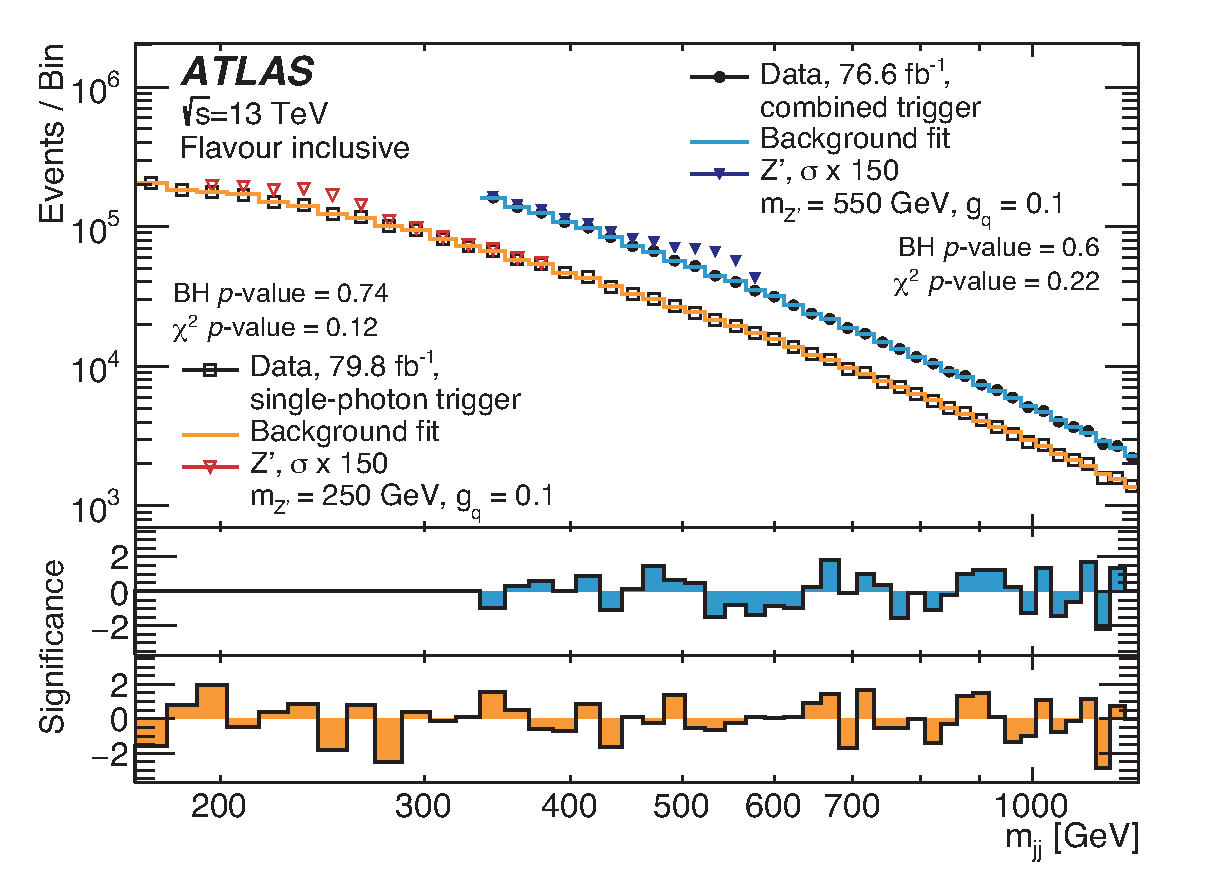
\includegraphics[width=\textwidth]{figures/chapter_dijet/figure1_inclusive_withTrigLabels_noBumpLimits}
    \caption{\label{fig:1a}}
  \end{subfigure}
  \begin{subfigure}[b]{0.49\textwidth}
    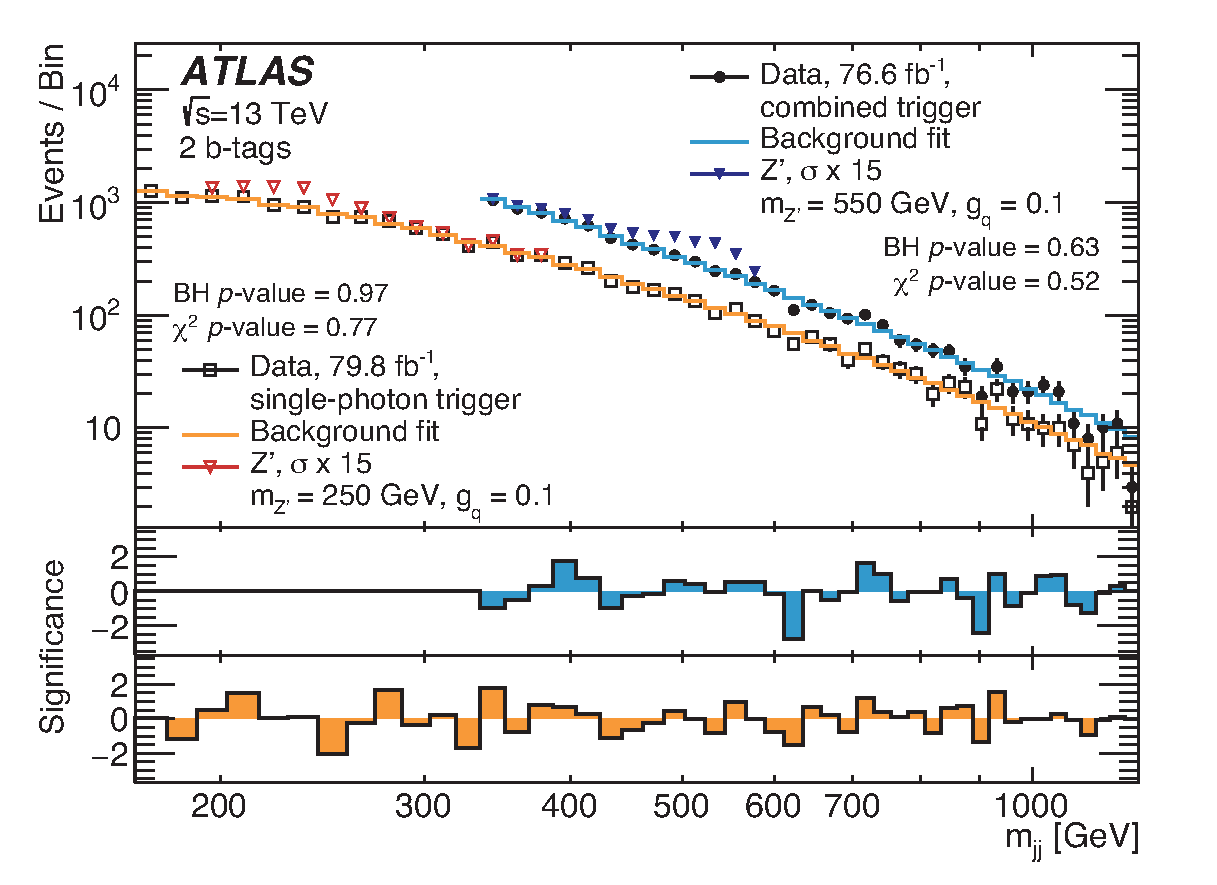
\includegraphics[width=\textwidth]{figures/chapter_dijet/figure1_nbtag2_withTrigLabels_noBumpLimits}
    \caption{\label{fig:1b}}
  \end{subfigure}
  \caption[]{Dijet mass distributions for the \subref{fig:1a} flavour-inclusive and \subref{fig:1b} \btagged categories.
  In both figures, the distribution for the sample collected using the combined trigger with $\photonPt > 95\,\GeV$ and two $\jetPt > 25\,\GeV$ jets (filled circles) and the distribution for the sample collected using the single-photon trigger with $\photonPt > 150\,\GeV$  (open squares) are shown separately. 
  The solid lines indicate the background estimated from the fitting method described in the text.
%    For the flavour-inclusive distributions, the method uses the 5 parameter variant of Eq.~(\ref{eq:5par}) in the single-photon triggered case and the 4 parameter variant of Eq.~(\ref{eq:5par}) in the combined trigger case.
%    In the \btagged categories, the method uses the 4 parameter variant of Eq.~(\ref{eq:5par}) in the single-photon triggered case and the 3 parameter variant of Eq.~(\ref{eq:5par}) in the combined trigger case.
    Also shown are 
    %the most-discrepant mass interval identified by \BumpHunter\ (dashed vertical lines) and 
    the $p$-values  both by a $\chi^2$ comparison of data to background estimate and by \BumpHunter (BH). 
    The solid and empty triangles represent a $\Zprime$ injected signal with \gq = 0.1, masses of 550 and 250~\GeV, respectively, where the theory-cross section is multiplied by the factor shown in the legend.
    The bottom panels show the significances of bin-by-bin differences between the data and the fits for the combined trigger (middle) and single-photon trigger (bottom).
    These Gaussian significances are calculated from the Poisson probability, considering only statistical uncertainties on the data.
  }
  \label{fig:data}
\end{figure}


\section{Search results}
\label{sec:result}
%-------------------------------------------------------------------------------

Fig.~\ref{fig:data} shows the results of fitting each of the observed distributions, as described in Section~\ref{sec:background}.
For each distribution, the function among those in Eqs.~(\ref{eq:ua2}) and (\ref{eq:5par}) and their variants which yields the highest $\chi^2$ $p$-value (shown in the figure), in absence of localized excesses, is chosen as the primary function for the fitting method.
The function with the lowest $\chi^2$ $p$-value which still results in a $p$-value larger than 0.05 is chosen as an alternative function.
The primary and alternative functions for each of the four search categories are shown in Table~\ref{tab:fitsummary}.
The alternative function is used to estimate the systematic uncertainty of the background prediction due to the choice of function, as described below.

%%%%%%%%%%%%%%%%%%%%%%
% Summary of fit functions

\begin{table}
  \caption[]{Summary of functions used for background fits to each category.
    The five-parameter function (5~par.) is given in Eq.~(\ref{eq:5par}).
    The four-parameter variant (4~par.) sets $p_5 = 0$, while the three-parameter variant (3~par) sets $p_5 = p_4 = 0$.}
    %The UA2 function is given by Eq.~(\ref{eq:ua2}). 
  \begin{tabularx}{\textwidth}{ l | *4{>{\centering\arraybackslash}X}@{}}
    \toprule
    \centering
		Fit               						        & Flavour-inclusive, single~$\gamma$~trigger     & Flavour-inclusive, combined~trigger 			& \btagged, single~$\gamma$~trigger   		   & \btagged, combined~trigger.        \\ \midrule
        Primary fit 								    & Eq.~(\ref{eq:5par}), 5~par.   & Eq.~(\ref{eq:5par}), 4~par. & Eq.~(\ref{eq:5par}), 4~par. & Eq.~(\ref{eq:5par}), 3~par. \\
        ($\chi^2$ $p$-value)       						& (0.11) 					    & (0.23)  					  &  (0.75)  				    & (0.53) 					  \\ \midrule
        Alternative fit 							    & Eq.~(\ref{eq:5par}), 4~par.	& Eq.~(\ref{eq:ua2}) 		  & Eq.~(\ref{eq:5par}), 3~par. & Eq.~(\ref{eq:5par}), 5~par.\\ 
 	    ($\chi^2$ $p$-value)       						& (0.07) 					    & (0.20)  					  &  (0.75)  				    & (0.44) 					  \\ \bottomrule
 	\end{tabularx}
    \label{tab:fitsummary}
\end{table}

%% In all cases the fits agree with the observed data with a  $p$-value above $0.5$.
%% The lower panels of the figure show the significances of bin-by-bin differences between the data and the fits. These Gaussian significances are calculated from the Poisson probability considering only statistical uncertainties. The data have been overlaid with examples of the signals described in Sec.~\ref{sec:samples}.
The statistical significance of any localised excess in each $\mjj$ distribution is quantified using the \BumpHunter~(BH) algorithm~\cite{Aaltonen:2008vt,Choudalakis:2011bh}.
The algorithm compares the binned $\mjj$ distribution of the data with the fitted background estimate, considering mass intervals centered in each bin location and with widths of variable size from two bins up to half the mass range used for the search (169 or 335 GeV to 1.1 TeV, for the single and combined trigger respectively). 
%In Figure~\ref{fig:data}, the region labelled \emph{\BumpHunter\ interval} depicts the most discrepant interval found for each distribution.

The statistical significance of the outcome is evaluated using the ensemble of possible outcomes by applying the algorithm to many pseudo-data samples drawn randomly from the background fit.
Without including systematic uncertainties, the \BumpHunter\ $p$-value -- the probability that fluctuations of the background model would produce an excess at least as significant as the one observed in the data, anywhere in the distribution -- is $p > 0.5$ for all distributions.
Thus, there is no evidence of a localised contribution to the mass distribution from new phenomena.

\section{Limit setting}
\label{sec:dijetlimits}

Limits are set on the possible contributions to the $\mjj$ distributions from two kinds of resonant signal processes.
As a specific benchmark signal, a leptophobic $\Zprime$ resonance is simulated as in Refs.~\cite{LHCDMF:2015,EXOT-2015-02}.
The $\Zprime$ resonance has axial-vector couplings to quarks and to a fermion dark-matter candidate.
The coupling of the $\Zprime$ to quarks, $\gq$, is set to be universal in quark flavour.
The mass of the dark-matter fermion is set to a value much heavier than the $\Zprime$, such that the decay width to dark matter is zero.
The total width $\Gamma_{\Zprime}$ is computed as the minimum width allowed given the coupling and mass $m_{\Zprime}$; this width is $3.6\%$--$4.2\%$ of the mass for $m_{\Zprime}=0.25$--$0.95$~\TeV and $\gq=0.3$. 
The interference between the $\Zprime$ in this benchmark model and the Standard Model $Z$ boson is assumed to be negligible.
A set of event samples were generated at leading order with $m_{\Zprime}$ values in the range 0.25--1.5~\TeV and with $\gq=0.3$ using \MGMCatNLOV{2.2.3}~\cite{Alwall:2014hca}; the \textsc{NNPDF3.0 LO} PDF set~\cite{Ball:2012cx} was used in conjunction with \PYTHIA~8.186~\cite{Sjostrand:2007gs} and the \textsc{A14} set of tuned parameters~\cite{ATL-PHYS-PUB-2014-021}.
For these samples, the acceptances of the kinematic selections in the flavour-inclusive categories range from 1\% to 2.5\%, increasing with signal mass, for the sample collected by the combined trigger and from 4\% to 10\% for the sample collected by the single-photon trigger. 
For the \btagged categories, the kinematic acceptance is defined relative to the full flavour-inclusive generated samples, leading to acceptance values of 0.2\%--0.4\% and 0.7\%--1.6\% for the combined and single-photon trigger, respectively. 
The reconstruction efficiencies range from 74\% to 80\% for the flavour-inclusive categories and from 40\% to 48\% for the \btagged categories, decreasing with increasing signal mass.

%In each search, a Bayesian method with a constant prior is applied to the $\mjj$ data and simulation of signals for discrete mass values to set 95\% credibility-level (CL) upper limits on the cross-section times acceptance for the signals described above~\cite{EXOT-2010-07}.
Limits are set on the considered new-physics contributions to the $\mjj$ distributions using a Bayesian method. 
A constant prior is used for the signal cross-section and Gaussian priors for nuisance parameters corresponding to systematic uncertainties. 
The expected limits are calculated using pseudo-experiments generated from the background-only component of a signal-plus-background fit to the data, using the same fitting ranges and functions selected as the best model in the search phase.  
Signal hypotheses at discrete mass values are used to set 95\% credibility-level (CL) upper limits on the cross-section times acceptance ~\cite{EXOT-2010-07}.
The limits are obtained for a discrete set of points in the $\gq$--$m_{\Zprime}$ plane, shown in Fig.~\ref{fig:limits_zprime}. 
 %% The signal mass range probed by the $X+\gamma$ search ranges from 250 GeV to 950 GeV, while the mass range for the  $X+j$ search spans 350 to 550 GeV. In both searches, the choice of mass points ensures that the presence of signal does not bias the background estimation. In the case of the $X+j$ search, the sensitivity to signal masses above 550 GeV is reduced by the increasing number of events where the subleading and third leading jets do not correspond to the decay  products of the  $\Zprime$. For the $\Zprime$ model considered above, the acceptance is \SignalAcceptanceForMassPointGamma\% for $m_{\Zprime}=350$~\GeV~and a coupling of $\gq$ = 0.3 in the $X+\gamma$ search, and \SignalAcceptanceForMassPointJet\% for the same benchmark point in the $X+j$ search.

\begin{figure}
  \centering
  \begin{subfigure}[b]{0.49\textwidth}
	  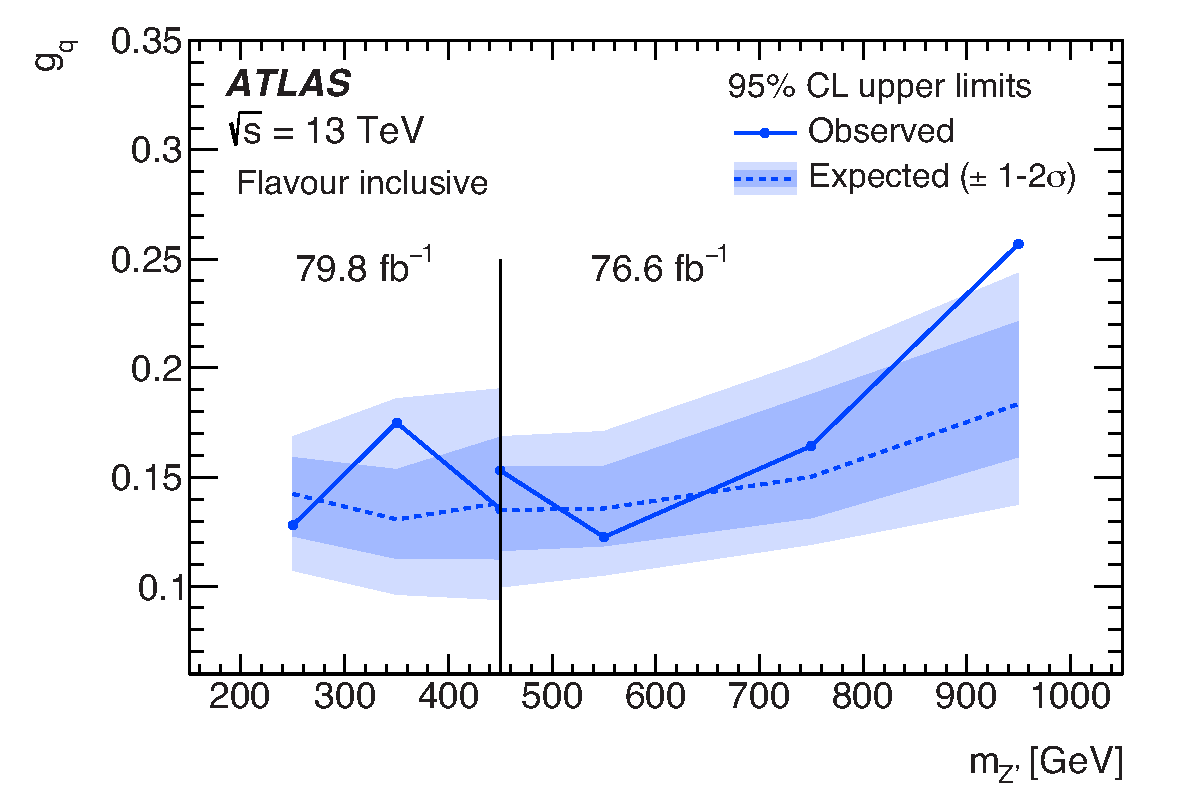
\includegraphics[width=\textwidth]{figures/chapter_dijet//2dlimits/Limits_2D_inclusive.pdf}
%	\caption{Flavour-inclusive}
	\caption{\label{fig:limit_single_inc_0p2}}
  \end{subfigure}
  \begin{subfigure}[b]{0.49\textwidth}
	  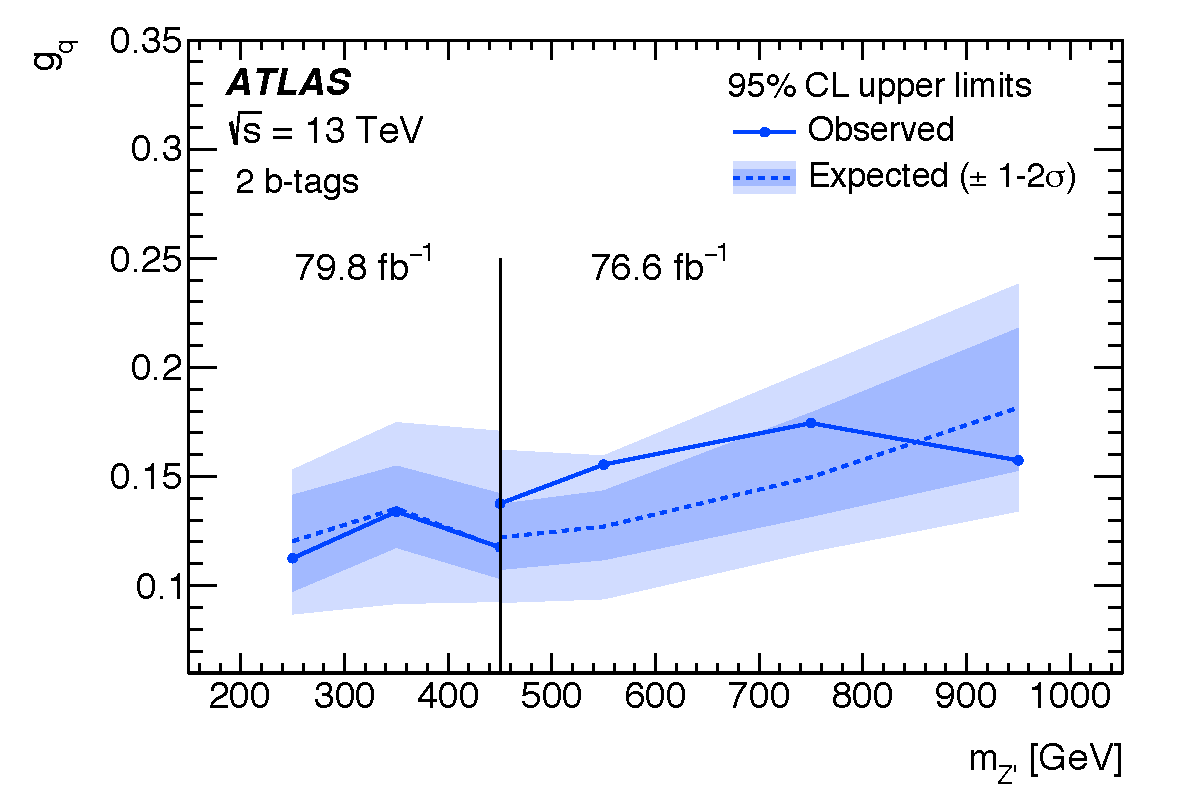
\includegraphics[width=\textwidth]{figures/chapter_dijet//2dlimits/Limits_2D_btagged.pdf}
%	\caption{\btagged}
    \caption{\label{fig:limit_single_btag_0p2}}

  \end{subfigure} \\
  \caption[Upper limits on $\Zprime$ contributions]{
    Excluded values of the coupling between a $\Zprime$ and quarks, at 95\% CL, as a function of $m_{\Zprime}$, from \subref{fig:limit_single_inc_0p2} the flavour-inclusive and \subref{fig:limit_single_btag_0p2} the \btagged categories.
    Below $450\,\GeV$ the distribution of events selected by the single-photon trigger is used for hypothesis testing, while above $450\,\GeV$ the combined trigger is used.} \label{fig:limits_zprime}
\end{figure}

\begin{figure}
  \centering
  \begin{subfigure}[b]{0.49\textwidth}
    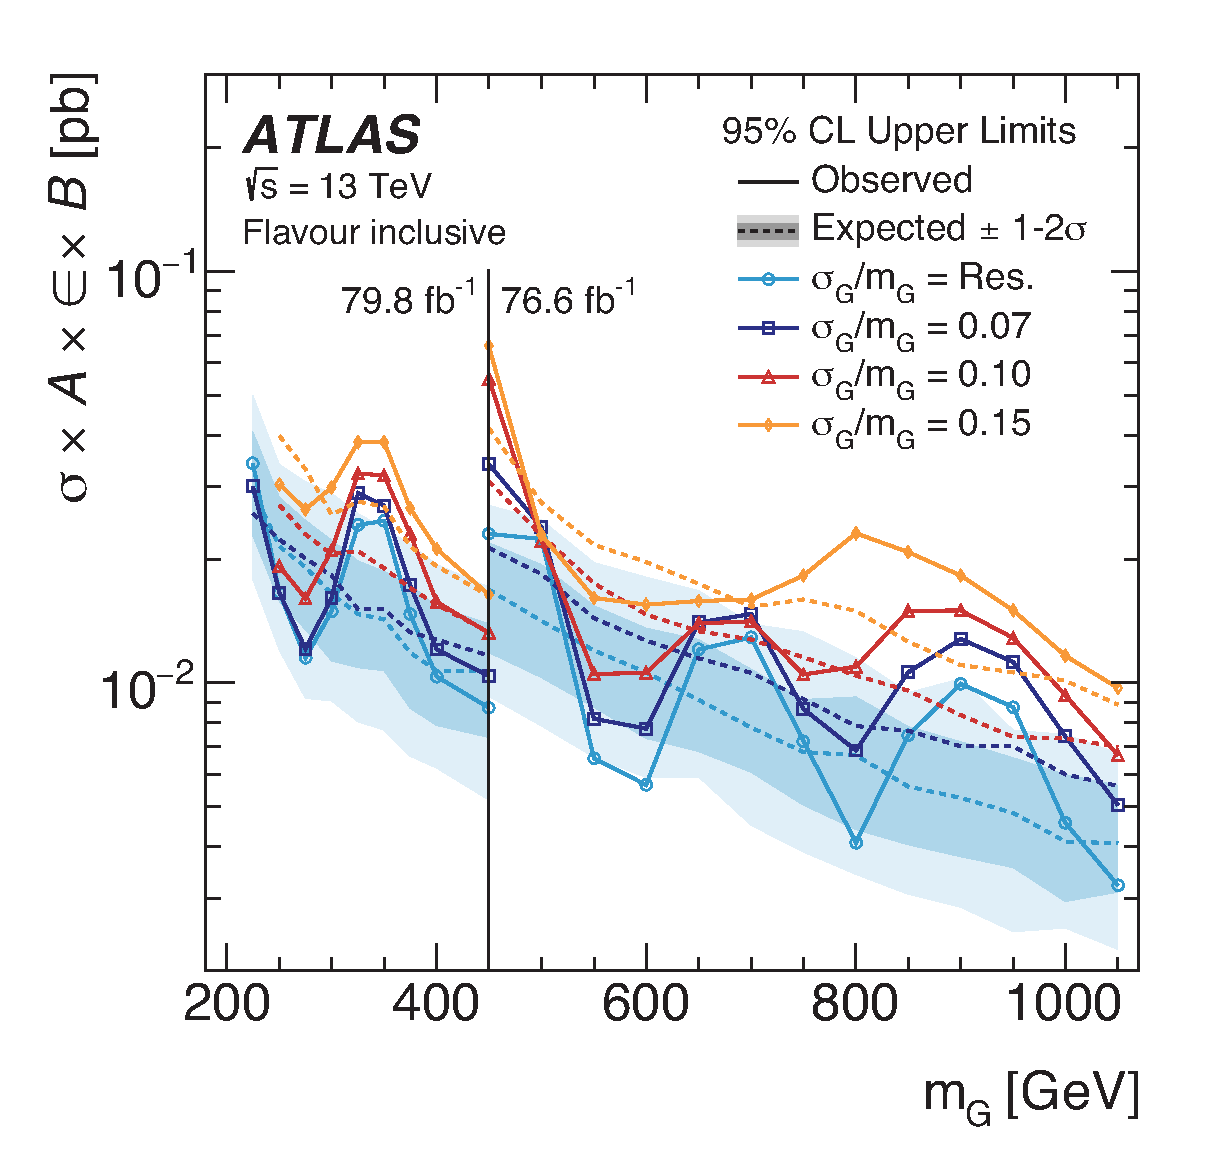
\includegraphics[width=\textwidth]{figures/chapter_dijet/GenericGaussians_CombinedInc}
	  %% \caption{Flavour-inclusive}
	  \caption{\label{fig:limit_gaussian_inc}}
  \end{subfigure}
  \begin{subfigure}[b]{0.49\textwidth}
    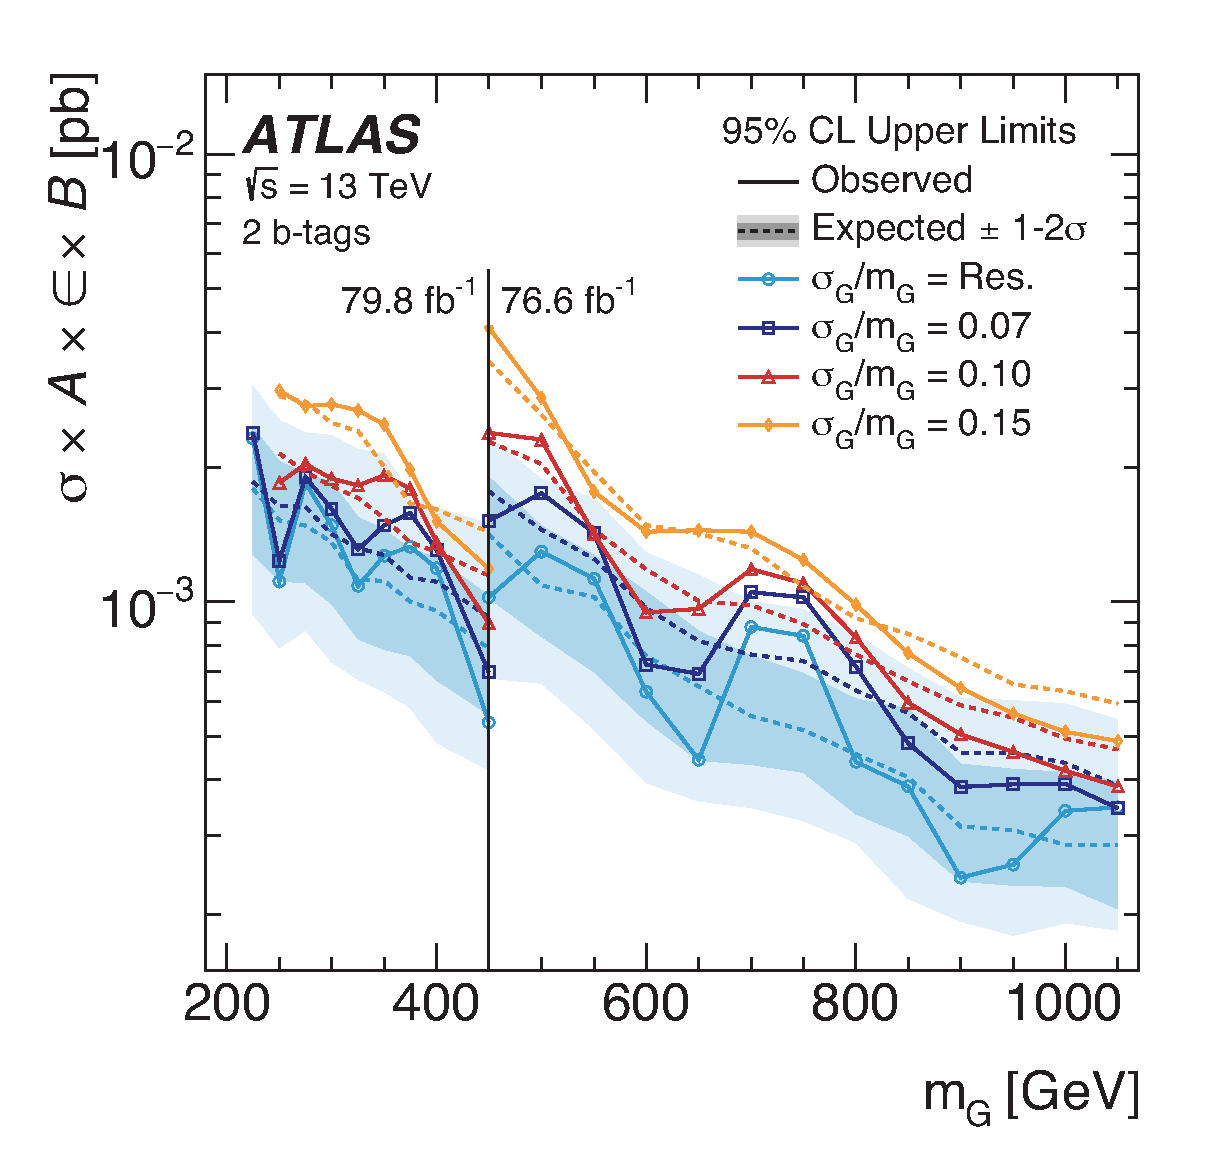
\includegraphics[width=\textwidth]{figures/chapter_dijet/GenericGaussians_Combined2b}
	  %% \caption{\btagged}
	  \caption{\label{fig:limit_gaussian_btag}}
  \end{subfigure}
  \caption[]{Upper limits on Gaussian-shape contributions to the dijet mass distributions from \subref{fig:limit_gaussian_inc} the flavour-inclusive and \subref{fig:limit_gaussian_btag} the \btagged categories.
    The curve denoted ``Res.'' represents the limit on intrinsically narrow contributions with Gaussian mass resolution ranging from 8\% to 3\% for the mass range considered.
    Below $450\,\GeV$, the distribution of events selected by the single-photon trigger is used for hypothesis testing, while above $450\,\GeV$ the combined trigger category is used.
    While the vertical axis is shared between the two selections, the signal acceptance is not the same below and above the line, and this results in different limits for the $450\,\GeV$ resonance mass point. 
    Thus the two sets of limit points correspond to two different interpretations of the product of cross-section, acceptance, efficiency, and branching ratio, $\sigma \times A \times \epsilon \times \mathcal{B}$.}
  \label{fig:limits_gaussian}
\end{figure}

%The limit setting method uses a constant prior for the signal cross-section and Gaussian priors for nuisance parameters corresponding to systematic uncertainties.
%The expected limits are calculated using pseudo-experiments generated from these priors, centred around the best fit model from the search phase.

%% The limits on the coupling $\gq$ are obtained from the cross-section limits on nearby discrete model points using the fact that the signal cross-section scales with $\gq^2$.

A more generic set of limits is shown in Fig.~\ref{fig:limits_gaussian}. These limits apply to the visible cross-section from a Gaussian-shape contribution to the $\mjj$ distribution, where the visible cross-section is defined as the product of the production cross-section, the detector acceptance, the reconstruction efficiency, and the branching ratio, $\sigma \times A \times \epsilon \times \mathcal{B}$.
The Gaussian-shape contributions have mass $m_\mathrm{G}$ and widths that span from the detector mass resolution, denoted ``Res.'' in the figure, ranging from 8\% to 3\% for the mass range considered, for an intrinsically narrow resonance, up to 15\% of the mean of the Gaussian mass distribution.

%% Limits are set only when $m_G$ is within at least twice the width of the Gaussian from the endpoints of this range.

%% This places 95\% CL upper limits on the cross-section times acceptance (visible cross-section) for new processes producing a photon or a jet and a resonance jet pair.
%% As the width increases, the expected signal contribution is distributed across more bins.
%% Therefore wider signals are affected less than narrower signals by statistical fluctuations of the data in a single bin. The searches have reduced sensitivity to wider signals compared to narrower signals.

%% For sufficiently narrow resonances, the results obtained for Gaussian signals may be used to set limits in BSM models beyond the one considered explicitly in this note. 
%% These limits can be used when off-peak contributions to the reconstructed $\mjj$ distribution predicted by the BSM model, such as those due to jet-combinatorics, PDF, and non-perturbative effects~\cite{Harris:2011bh}, can be safely neglected or truncated, leaving a Gaussian core. This is the case of the  $\Zprime$ axial vector signals used as benchmark in these searches. Signals with an intrinsic width much smaller than 5\% should be compared to the limit curve for a width equal to the experimental resolution.
%% Predicted signals with larger widths should be compared with the limit that corresponds most closely to the width of the Gaussian contribution predicted by the model.
%% More instructions can be found in Appendix A of Ref.~\cite{EXOT-2013-11}.

Both the choice of fit function and statistical fluctuations in the $\mjj$ distribution can contribute to uncertainties in the background model.
To account for the fit function choice, the largest difference between fits among the variants of Eq.~(\ref{eq:ua2}) and~ Eq.~(\ref{eq:5par}) that obtain a $p$-value above 0.05, is taken as a systematic uncertainty.
The uncertainty related to statistical fluctuations in the background model is computed via Poisson fluctuations around the values of the nominal background model.
The uncertainty of the prediction in each $\mjj$ bin is taken to be the standard deviation of the predictions from all random samples.

The reconstructed signal mass distributions are affected by additional uncertainties related to the simulation of detector effects.
The jet energy scale uncertainty is applied to the $\Zprime$ mass distributions using a four-principal-component method~\cite{PERF-2016-04,ATL-PHYS-PUB-2015-014,ATL-PHYS-PUB-2015-015}, leading to an average 2\% shift of the peak value for each mass distribution.
For the Gaussian-shape signal models, this average 2\% shift is taken as the uncertainty of the mean of each Gaussian distribution.
In the case of the \btagged\ categories, uncertainties of the \btagging\ efficiency are the dominant uncertainties in each mass distribution.
To account for these uncertainties, the contribution of each simulated event to a given mass distribution is reweighted by 5\%--15\% for each jet, depending on its $\pt$~\cite{PERF-2016-05}.

The remaining uncertainties are modelled by scaling each simulated distribution by 3\% to account for jet energy resolution in all categories~\cite{PERF-2016-04}, 2\% for photon identification uncertainties in the single-photon-trigger categories and 1.4\% in the combined-trigger categories~\cite{PERF-2017-02}, 3\% to account for efficiencies of the combined trigger, and 1\% for PDF-related uncertainties (only applied to the mass distributions of $\Zprime$ signals).

All these uncertainties are included in the reported limits; further uncertainties of the theoretical cross-section for the \Zprime model are not considered.

The uncertainty of the combined 2015--2017 integrated luminosity is derived following a methodology similar to that detailed in Ref.~\cite{DAPR-2013-01} and using the LUCID-2 detector for the baseline luminosity measurements in 2017~\cite{LUCID2}.
The estimates for the individual datasets are combined and applied as a single scaling parameter with a value of 2\% for the single-photon-trigger categories and 2.3\% for the combined-trigger categories.

%-------------------------------------------------------------------------------
\section{Conclusion}
%% \label{sec:conclusion}
%-------------------------------------------------------------------------------

Dijet resonances with a width up to 15\% of the mass, produced in association with a photon, were searched for in up to $79.8\,\ifb$ of LHC $pp$ collisions recorded by the ATLAS experiment at $\sqrt{s}=13\,\TeV$. The observed $\mjj$ distribution in the mass range $169\,\GeV < \mjj < 1100\,\GeV$ can be described by a fit with smooth functions without contributions from such resonances.

%no significant evidence of resonant phenomena beyond the Standard Model is seen in the mass range $225\,\GeV < \mjj < 1100\,\GeV$.

In the absence of a statistically significant excess, limits are set on two models: $\Zprime$ axial-vector dark-matter mediators and Gaussian-shape signal contributions.
All mediator masses within the analysis range are excluded for a coupling value of $\gq = 0.25$ and above, with the exclusion limit near a coupling of $\gq=0.15$ for most of the mass range.
The \btagged categories yield $\Zprime$ limits comparable to the flavour-inclusive categories, assuming that the $\Zprime$ decays equally into all quark flavours, and provide model-independent limits that can be reinterpreted in terms of resonances decaying preferentially into $b$-quarks.
For narrow Gaussian-shape structures with a width-to-mass ratio of 7\%, the flavour-inclusive categories exclude visible cross-sections above 12~fb for a mass of 400~\GeV and above 5.1~fb for a mass of 1050~\GeV.
When wider signals with a width-to-mass ratio of 15\% are considered, the exclusion limits are weaker at the lower mass values, with visible cross-sections above 21~fb excluded for a mass of $400\,\GeV$ and those above 9.7~fb excluded for a mass of $1050\,\GeV$. 

These results significantly extend the constraints by ATLAS and other experiments at lower centre-of-mass energies on hadronically decaying resonances with masses as low as 225 GeV and up to 1100 GeV.




